% Generated by julia/scripts/generate_figure_audit_artifacts.jl.
% Exact sources: unified_elasticity_switching_v1_{capacity,penalized_path}.csv.
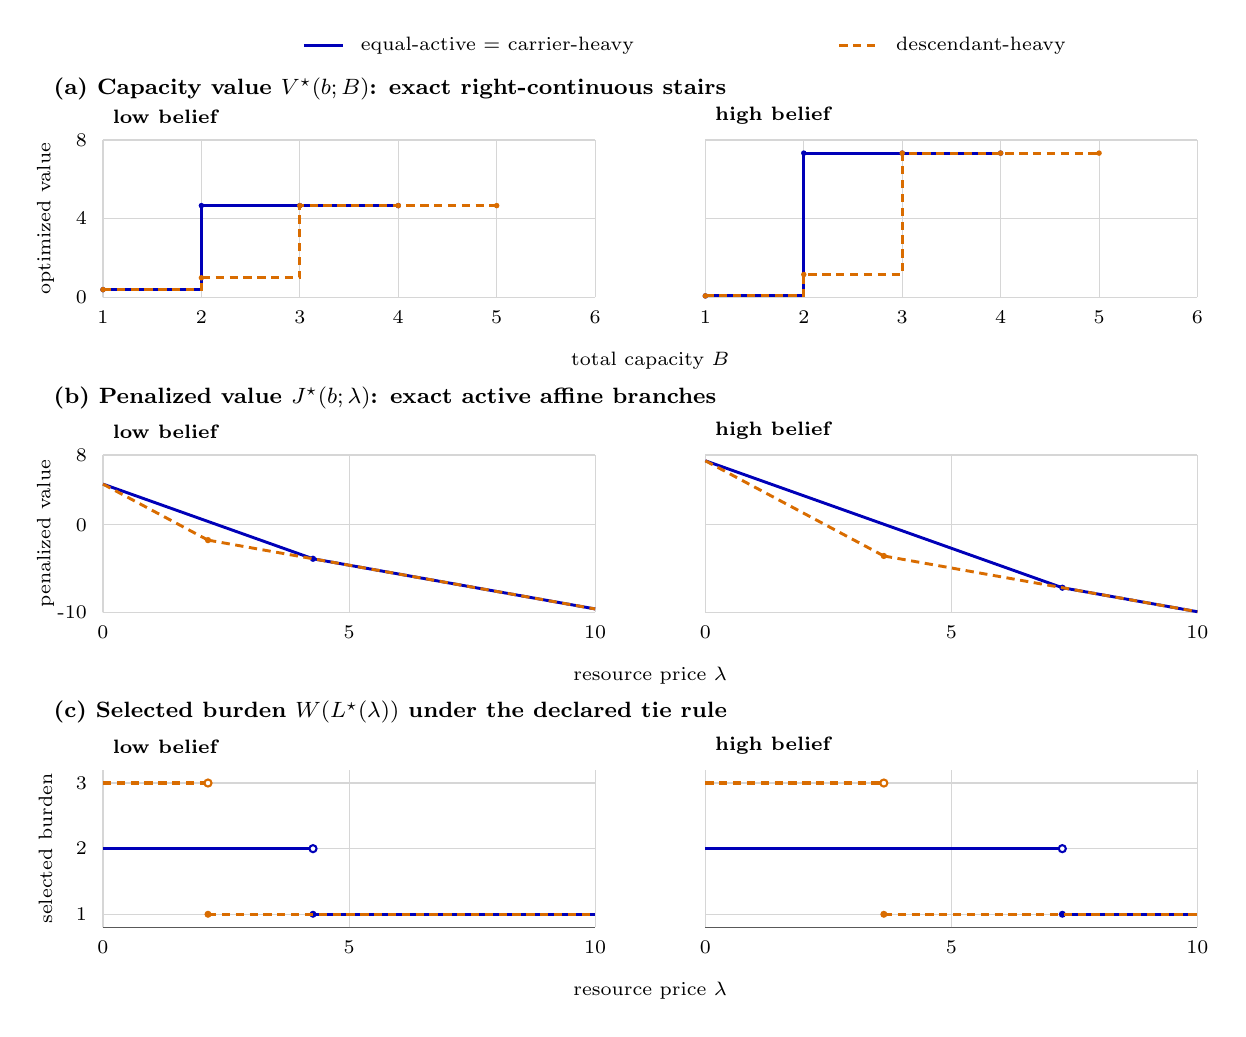
\begin{tikzpicture}[x=1cm,y=1cm,font=\scriptsize]
  \draw[blue!72!black,line width=1.05pt] (3.55,10.95) -- (4.05,10.95);
  \node[anchor=west] at (4.15,10.95) {equal-active = carrier-heavy};
  \draw[orange!85!black,densely dashed,line width=1.05pt] (10.35,10.95) -- (10.85,10.95);
  \node[anchor=west] at (10.95,10.95) {descendant-heavy};
  \node[font=\bfseries\footnotesize,anchor=west] at (0.25,10.40) {(a) Capacity value \(V^\star(b;B)\): exact right-continuous stairs};
  \node[font=\bfseries\scriptsize,anchor=south west] at (1.0,9.83) {low belief};
  \draw[black!65] (1.0,7.75) -- (7.25,7.75);
  \draw[black!65] (1.0,7.75) -- (1.0,9.75);
  \draw[black!16] (1.0,7.75) -- (1.0,9.75);
  \node[anchor=north,font=\scriptsize] at (1.0,7.7) {1};
  \draw[black!16] (2.25,7.75) -- (2.25,9.75);
  \node[anchor=north,font=\scriptsize] at (2.25,7.7) {2};
  \draw[black!16] (3.5,7.75) -- (3.5,9.75);
  \node[anchor=north,font=\scriptsize] at (3.5,7.7) {3};
  \draw[black!16] (4.75,7.75) -- (4.75,9.75);
  \node[anchor=north,font=\scriptsize] at (4.75,7.7) {4};
  \draw[black!16] (6.0,7.75) -- (6.0,9.75);
  \node[anchor=north,font=\scriptsize] at (6.0,7.7) {5};
  \draw[black!16] (7.25,7.75) -- (7.25,9.75);
  \node[anchor=north,font=\scriptsize] at (7.25,7.7) {6};
  \draw[black!16] (1.0,7.75) -- (7.25,7.75);
  \node[anchor=east,font=\scriptsize] at (0.92,7.75) {0};
  \draw[black!16] (1.0,8.75) -- (7.25,8.75);
  \node[anchor=east,font=\scriptsize] at (0.92,8.75) {4};
  \draw[black!16] (1.0,9.75) -- (7.25,9.75);
  \node[anchor=east,font=\scriptsize] at (0.92,9.75) {8};
  \draw[blue!72!black,solid,line width=1.05pt] (1.0,7.84983) -- (2.25,7.84983) -- (2.25,8.91667) -- (3.5,8.91667) -- (3.5,8.91667) -- (4.75,8.91667) -- (4.75,8.91667);
  \fill[blue!72!black] (1.0,7.84983) circle (0.035);
  \fill[blue!72!black] (2.25,8.91667) circle (0.035);
  \fill[blue!72!black] (3.5,8.91667) circle (0.035);
  \fill[blue!72!black] (4.75,8.91667) circle (0.035);
  \draw[orange!85!black,densely dashed,line width=1.05pt] (1.0,7.84983) -- (2.25,7.84983) -- (2.25,8.0) -- (3.5,8.0) -- (3.5,8.91667) -- (4.75,8.91667) -- (4.75,8.91667) -- (6.0,8.91667) -- (6.0,8.91667);
  \fill[orange!85!black] (1.0,7.84983) circle (0.035);
  \fill[orange!85!black] (2.25,8.0) circle (0.035);
  \fill[orange!85!black] (3.5,8.91667) circle (0.035);
  \fill[orange!85!black] (4.75,8.91667) circle (0.035);
  \fill[orange!85!black] (6.0,8.91667) circle (0.035);
  \node[font=\bfseries\scriptsize,anchor=south west] at (8.65,9.83) {high belief};
  \draw[black!65] (8.65,7.75) -- (14.9,7.75);
  \draw[black!65] (8.65,7.75) -- (8.65,9.75);
  \draw[black!16] (8.65,7.75) -- (8.65,9.75);
  \node[anchor=north,font=\scriptsize] at (8.65,7.7) {1};
  \draw[black!16] (9.9,7.75) -- (9.9,9.75);
  \node[anchor=north,font=\scriptsize] at (9.9,7.7) {2};
  \draw[black!16] (11.15,7.75) -- (11.15,9.75);
  \node[anchor=north,font=\scriptsize] at (11.15,7.7) {3};
  \draw[black!16] (12.4,7.75) -- (12.4,9.75);
  \node[anchor=north,font=\scriptsize] at (12.4,7.7) {4};
  \draw[black!16] (13.65,7.75) -- (13.65,9.75);
  \node[anchor=north,font=\scriptsize] at (13.65,7.7) {5};
  \draw[black!16] (14.9,7.75) -- (14.9,9.75);
  \node[anchor=north,font=\scriptsize] at (14.9,7.7) {6};
  \draw[black!16] (8.65,7.75) -- (14.9,7.75);
  \draw[black!16] (8.65,8.75) -- (14.9,8.75);
  \draw[black!16] (8.65,9.75) -- (14.9,9.75);
  \draw[blue!72!black,solid,line width=1.05pt] (8.65,7.76997) -- (9.9,7.76997) -- (9.9,9.58333) -- (11.15,9.58333) -- (11.15,9.58333) -- (12.4,9.58333) -- (12.4,9.58333);
  \fill[blue!72!black] (8.65,7.76997) circle (0.035);
  \fill[blue!72!black] (9.9,9.58333) circle (0.035);
  \fill[blue!72!black] (11.15,9.58333) circle (0.035);
  \fill[blue!72!black] (12.4,9.58333) circle (0.035);
  \draw[orange!85!black,densely dashed,line width=1.05pt] (8.65,7.76997) -- (9.9,7.76997) -- (9.9,8.04167) -- (11.15,8.04167) -- (11.15,9.58333) -- (12.4,9.58333) -- (12.4,9.58333) -- (13.65,9.58333) -- (13.65,9.58333);
  \fill[orange!85!black] (8.65,7.76997) circle (0.035);
  \fill[orange!85!black] (9.9,8.04167) circle (0.035);
  \fill[orange!85!black] (11.15,9.58333) circle (0.035);
  \fill[orange!85!black] (12.4,9.58333) circle (0.035);
  \fill[orange!85!black] (13.65,9.58333) circle (0.035);
  \node[anchor=north] at (7.95,7.18) {total capacity \(B\)};
  \node[rotate=90] at (0.27,8.75) {optimized value};
  \node[font=\bfseries\footnotesize,anchor=west] at (0.25,6.48) {(b) Penalized value \(J^\star(b;\lambda)\): exact active affine branches};
  \node[font=\bfseries\scriptsize,anchor=south west] at (1.0,5.83) {low belief};
  \draw[black!65] (1.0,3.75) -- (7.25,3.75);
  \draw[black!65] (1.0,3.75) -- (1.0,5.75);
  \draw[black!16] (1.0,3.75) -- (1.0,5.75);
  \node[anchor=north,font=\scriptsize] at (1.0,3.7) {0};
  \draw[black!16] (4.125,3.75) -- (4.125,5.75);
  \node[anchor=north,font=\scriptsize] at (4.125,3.7) {5};
  \draw[black!16] (7.25,3.75) -- (7.25,5.75);
  \node[anchor=north,font=\scriptsize] at (7.25,3.7) {10};
  \draw[black!16] (1.0,3.75) -- (7.25,3.75);
  \node[anchor=east,font=\scriptsize] at (0.92,3.75) {-10};
  \draw[black!16] (1.0,4.86111) -- (7.25,4.86111);
  \node[anchor=east,font=\scriptsize] at (0.92,4.86111) {0};
  \draw[black!16] (1.0,5.75) -- (7.25,5.75);
  \node[anchor=east,font=\scriptsize] at (0.92,5.75) {8};
  \draw[blue!72!black,solid,line width=1.05pt] (1.0,5.37963) -- (3.6671,4.43133);
  \draw[blue!72!black,solid,line width=1.05pt] (3.6671,4.43133) -- (7.25,3.79437);
  \fill[blue!72!black] (3.6671,4.43133) circle (0.04);
  \draw[orange!85!black,densely dashed,line width=1.05pt] (1.0,5.37963) -- (2.33355,4.6684);
  \draw[orange!85!black,densely dashed,line width=1.05pt] (2.33355,4.6684) -- (7.25,3.79437);
  \fill[orange!85!black] (2.33355,4.6684) circle (0.04);
  \node[font=\bfseries\scriptsize,anchor=south west] at (8.65,5.83) {high belief};
  \draw[black!65] (8.65,3.75) -- (14.9,3.75);
  \draw[black!65] (8.65,3.75) -- (8.65,5.75);
  \draw[black!16] (8.65,3.75) -- (8.65,5.75);
  \node[anchor=north,font=\scriptsize] at (8.65,3.7) {0};
  \draw[black!16] (11.775,3.75) -- (11.775,5.75);
  \node[anchor=north,font=\scriptsize] at (11.775,3.7) {5};
  \draw[black!16] (14.9,3.75) -- (14.9,5.75);
  \node[anchor=north,font=\scriptsize] at (14.9,3.7) {10};
  \draw[black!16] (8.65,3.75) -- (14.9,3.75);
  \draw[black!16] (8.65,4.86111) -- (14.9,4.86111);
  \draw[black!16] (8.65,5.75) -- (14.9,5.75);
  \draw[blue!72!black,solid,line width=1.05pt] (8.65,5.67593) -- (13.18342,4.06404);
  \draw[blue!72!black,solid,line width=1.05pt] (13.18342,4.06404) -- (14.9,3.75887);
  \fill[blue!72!black] (13.18342,4.06404) circle (0.04);
  \draw[orange!85!black,densely dashed,line width=1.05pt] (8.65,5.67593) -- (10.91671,4.46701);
  \draw[orange!85!black,densely dashed,line width=1.05pt] (10.91671,4.46701) -- (14.9,3.75887);
  \fill[orange!85!black] (10.91671,4.46701) circle (0.04);
  \node[anchor=north] at (7.95,3.18) {resource price \(\lambda\)};
  \node[rotate=90] at (0.27,4.75) {penalized value};
  \node[font=\bfseries\footnotesize,anchor=west] at (0.25,2.48) {(c) Selected burden \(W(L^\star(\lambda))\) under the declared tie rule};
  \node[font=\bfseries\scriptsize,anchor=south west] at (1.0,1.83) {low belief};
  \draw[black!65] (1.0,-0.25) -- (7.25,-0.25);
  \draw[black!65] (1.0,-0.25) -- (1.0,1.75);
  \draw[black!16] (1.0,-0.25) -- (1.0,1.75);
  \node[anchor=north,font=\scriptsize] at (1.0,-0.3) {0};
  \draw[black!16] (4.125,-0.25) -- (4.125,1.75);
  \node[anchor=north,font=\scriptsize] at (4.125,-0.3) {5};
  \draw[black!16] (7.25,-0.25) -- (7.25,1.75);
  \node[anchor=north,font=\scriptsize] at (7.25,-0.3) {10};
  \draw[black!16] (1.0,-0.08333) -- (7.25,-0.08333);
  \node[anchor=east,font=\scriptsize] at (0.92,-0.08333) {1};
  \draw[black!16] (1.0,0.75) -- (7.25,0.75);
  \node[anchor=east,font=\scriptsize] at (0.92,0.75) {2};
  \draw[black!16] (1.0,1.58333) -- (7.25,1.58333);
  \node[anchor=east,font=\scriptsize] at (0.92,1.58333) {3};
  \draw[blue!72!black,solid,line width=1.15pt] (1.0,0.75) -- (3.6671,0.75);
  \draw[blue!72!black,solid,line width=1.15pt] (3.6671,-0.08333) -- (7.25,-0.08333);
  \draw[blue!72!black,line width=0.75pt,fill=white] (3.6671,0.75) circle (0.045);
  \fill[blue!72!black] (3.6671,-0.08333) circle (0.045);
  \draw[orange!85!black,densely dashed,line width=1.15pt] (1.0,1.58333) -- (2.33355,1.58333);
  \draw[orange!85!black,densely dashed,line width=1.15pt] (2.33355,-0.08333) -- (7.25,-0.08333);
  \draw[orange!85!black,line width=0.75pt,fill=white] (2.33355,1.58333) circle (0.045);
  \fill[orange!85!black] (2.33355,-0.08333) circle (0.045);
  \node[font=\bfseries\scriptsize,anchor=south west] at (8.65,1.83) {high belief};
  \draw[black!65] (8.65,-0.25) -- (14.9,-0.25);
  \draw[black!65] (8.65,-0.25) -- (8.65,1.75);
  \draw[black!16] (8.65,-0.25) -- (8.65,1.75);
  \node[anchor=north,font=\scriptsize] at (8.65,-0.3) {0};
  \draw[black!16] (11.775,-0.25) -- (11.775,1.75);
  \node[anchor=north,font=\scriptsize] at (11.775,-0.3) {5};
  \draw[black!16] (14.9,-0.25) -- (14.9,1.75);
  \node[anchor=north,font=\scriptsize] at (14.9,-0.3) {10};
  \draw[black!16] (8.65,-0.08333) -- (14.9,-0.08333);
  \draw[black!16] (8.65,0.75) -- (14.9,0.75);
  \draw[black!16] (8.65,1.58333) -- (14.9,1.58333);
  \draw[blue!72!black,solid,line width=1.15pt] (8.65,0.75) -- (13.18342,0.75);
  \draw[blue!72!black,solid,line width=1.15pt] (13.18342,-0.08333) -- (14.9,-0.08333);
  \draw[blue!72!black,line width=0.75pt,fill=white] (13.18342,0.75) circle (0.045);
  \fill[blue!72!black] (13.18342,-0.08333) circle (0.045);
  \draw[orange!85!black,densely dashed,line width=1.15pt] (8.65,1.58333) -- (10.91671,1.58333);
  \draw[orange!85!black,densely dashed,line width=1.15pt] (10.91671,-0.08333) -- (14.9,-0.08333);
  \draw[orange!85!black,line width=0.75pt,fill=white] (10.91671,1.58333) circle (0.045);
  \fill[orange!85!black] (10.91671,-0.08333) circle (0.045);
  \node[anchor=north] at (7.95,-0.82) {resource price \(\lambda\)};
  \node[rotate=90] at (0.27,0.75) {selected burden};
\end{tikzpicture}
